\section{Background}

This section contains basic knowledge that is necessary for the understanding of the rest of the thesis.
It briefly touches on artificial neural networks and convolutional neural networks in the beginning.
The subsection after that goes on to describe autoencoders in general. Next, Kullback-Leibler divergence
is explained in detail as it is an essential part for the variational autoencoders as they are used in this
work. Kullback-Leibler divergence also plays an important role in t-distributed stochastic neighbor embedding.
The difference between variational autoencoders and the standard undercomplete autoencoder is covered in the 
following subsection. Lastly, the dimensionality reduction method 
t-distributed stochastic neighbor embedding is discussed since it is used in this work to gain an 
understanding of the high dimensional latent space of the autoencoders.

\subsection{Remote Sensing Imagery}

%What are the challenges of remote sensing. The images are very big and high resolution and there is not a lot 
% of labeled data such as there is for common object for example COCO dataset

\subsection{Artificial Neuron}

The concept of neurons in computer science is inspired by biological neurons. An artificial neuron has one or
more weighted inputs that are summed together
and after that passed through a non-linear function called activation function. The output can then be used as
the input of another neuron similarly to how stronger or weaker connections can be formed in the biological
world.
By adjusting the separate weights of the inputs a single neuron is able to model
simple functions like the logic $and$ or the logic $or$ but it is not abled to solve other trivial problems
like the exclusive or (XOR).

\begin{figure}[h]
    \centering
    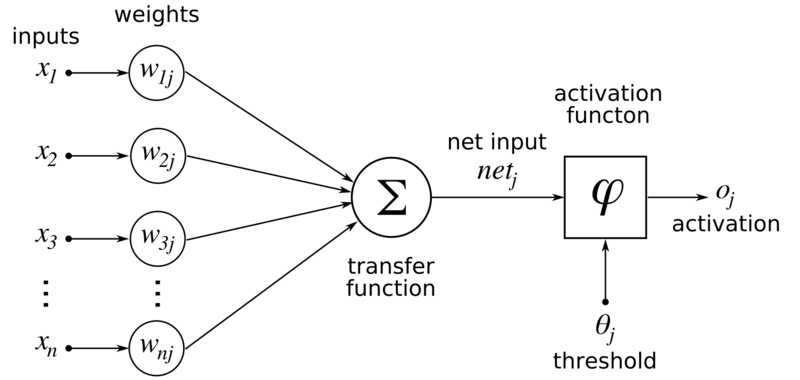
\includegraphics[width=0.7\textwidth]{images/figures/artificial_neuronHOML.png}
    \caption{An artificial neuron. Image taken from \parencite{2005-chrislb-artificial-neuron}}
\end{figure}


\subsection{Artificial Neural Network}

An artificial neural network (ANN) can model functions $f(x) = y$ with input and output vectors of any size.
This is done by assigning each value of the input vector $x$ to a single neuron. All those neurons together make
up the input layer of the ANN. The output layer of the ANN also has a single neuron for every value of the
output vector $y$. Between these input and output layers there can be multiple additional layers which are called
hidden layers. If there is at least one hidden layer, i.e. at least three layers in total, the ANN is abled to 
model arbitrarily complex functions given that the hidden layer can contain as many neurons as necessary.
However, in practice most of the time
deep neural networks with two or more hidden layers are used \parencite{2017-geron-homl}. 
If all the neurons of a previous layer are connected to each neuron in the following layer the layers are
called fully connected which is the case for every layer in the artificial neural network depicted
in Figure \ref{figure_fully_connected_nn}.

\begin{figure}[ht] 
    \centering
    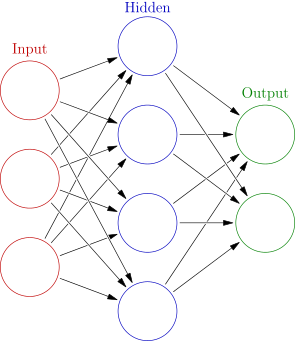
\includegraphics[width=0.3\textwidth]{images/figures/artificial_neural_network.png}
    \caption{An artificial neural network with three fully connected layers.
    Image taken from \parencite{2013-glosser-ann}} \label{figure_fully_connected_nn}
\end{figure} 

The process of learning an artificial neural networks $n(w, x)=\hat{y}$, with weights $w$, refers to the process
of iteratively adjusting $w$ in such a way that $n(w, x )$ more closely resembles the desired mapping  $f(x)=y$
that should be learned. This can be achieved by taking possible inputs $x_{i}$ for which the 
desired outputs $y_{i}$ are known and optimizing a so called loss function $l(n(w,x_{i}),y_{i})$ for $w$.
This loss function measures a difference between the desired output and the predictions for that output produced
by the ANN.
This process is then repeated with each pair of inputs $x_{i}$ and desired outputs $y_{i}$. The set of pairs of
those inputs and desired outputs is called the training set. 
Intuitively, the optimized loss function can be seen as the objective of how the output of the artificial neural
network should resemble the known desired outputs.

The optimization is most commonly done via gradient descent or adjusted versions of gradient descent.
This involves calculating the partial derivatives for each component of $w$.
For this reason the activation functions of the artificial neurons and the loss function have to be
differentiable. More detailed information about gradient descent can be read in Deep Learning
\parencite{2016-goodfellow-deep} and information about the commonly used optimizers that improve 
gradient descent can be found in Hands-On Machine Learning \parencite{2017-geron-homl}.

\subsection{Convolutional Neural Networks}

CNNs are especially good where the input has values that have to be interpreted in context to the other
inputs. This is for example the case in computer vision where the inputs are images whose
single pixel values have little
meaning if they are not in the context of their position relative to the other pixels. An example for
such a task, where CNNs perform well, is the classification of images of cats and dogs.
The difference of CNNs and fully connected networks is the use of convolutional layers.
A convolutional layer is not connected to every neuron of the previous layer but instead only to small
rectangle of neurons of the previous layer. For images this means that in the first convolutional layer
the neurons do not take every pixel of the image as input but instead only a small piece of the image.
This way a hierarchical structure is created where the first hidden layer learns lower level features
and the following layers learn ever higher level features. Also by only connecting a neuron to a few
neurons of the previous layer the number of weights is far lower which means there is much less memory
and time needed for training the network. That way computational expenditure is reduced in comparison
to fully connected layers.

The kernel of a layer is intuitively speaking the field of vision where a neuron takes its inputs from
the previous layer. If the kernel of a neuron laps over the edge
of the input space different kinds of padding can be used for the missing input values.
These kernels, also called filters, are basically matrices of weights that are
adjusted while training which way they learn features of the input. In practice multiple neurons have
the same input space leading to the ability to extract multiple features that can be processed
further in the following layer. The amount of neurons with the same input space is referred to as
the number of filters since each one of those neurons has its own filter with its respective
weights and all those filters are applied to the same piece of the input. This is visualized in
Figure \ref{figure_cnn_filter}.

\begin{figure}[h]
    \centering
    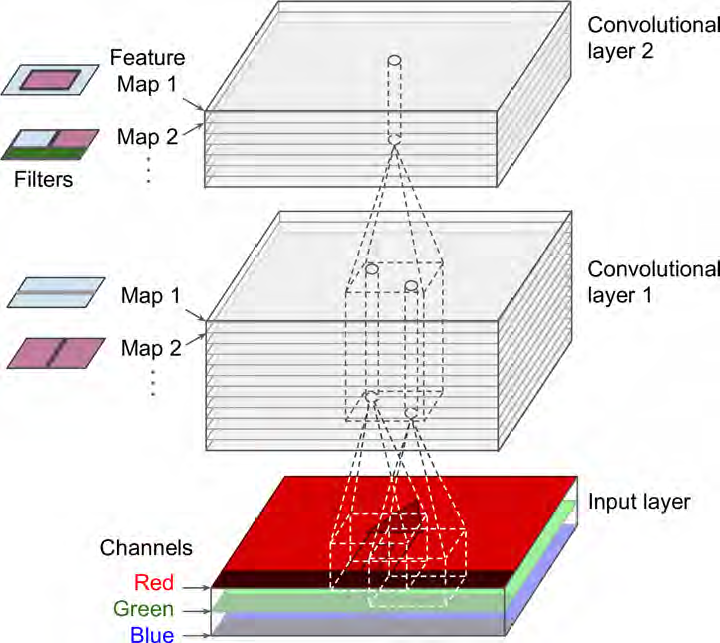
\includegraphics[width=0.6\textwidth]{images/figures/convolutional_net_multiple_filters.png}
    \caption{A convolutional network with 12 filters in the first convolutional layer and 7
    filters in the second convolutional layer. Each filters can learn different features and an
    RGB image is depicted as the input here.
    Image taken from \parencite{2017-geron-homl}} \label{figure_cnn_filter}
\end{figure}

Instead of having a kernel in each possible area of the input there can also be a distance between
each kernel which is called stride. This can be used to decrease the dimensionality of the output
of a layer. For example with strides of 2 the output dimensions are halve that of the input
dimensions.

\paragraph{Pooling}
A pooling layer replaces the value of an output with a summary of the nearby outputs. For instance
max pooling only takes the maximum output of all outputs in a surrounding rectangle. Note that
the pooling layers only perform an operation on multiple outputs of a previous layer and therefore
do not have weights. The use of pooling layers increases the networks tolerance to small changes in
the inputs \parencite{2016-goodfellow-deep} which is most of the time desired since the network should
learn features instead of exact pixel locations. Many popular CNN architectures like 
AlexNet \parencite{2012-krizhevsky-imagenet} use pooling layers between the convolutional layers.
In these CNNs the pooling layers are also often used to reduce the dimension of the layers.


\subsection{Autoencoders}

An autoencoder is an artificial neural network that aims to reproduce its input. The first part
of an autoencoder is the Encoder $f(x)=z$ that takes an input $x$ and maps it to a latent code $z$.
The second part is the decoder $g(z)=x'$ that tries to generate a reproduction $x'$ similar to the
input $x$ that the latent code $z$ was produced from. Since the output of the neural network should
be the same as the input there is no need for labeled data and the network can be learned unsupervised.
Just having a network that is the identity function would be useless but by constraining the autoencoder
in specific ways it can be forced to learn useful traits leading to possibilities in pretraining 
networks or randomly generating content similar to the content the autoencoder was trained with.

One common constraint for autoencoders is choosing a dimension for the latent code that is smaller
than the dimension of the input. This means that the encoder is forced to learn to extract only the
most important features from the input and the latent code is a representation of those most
important features in a lower dimensionality than the input. Such an autoencoder, called
undercomplete autoencoder, is visualized in Figure \ref{figure_undercomplete_ae}.

\begin{figure}[h]
    \centering
    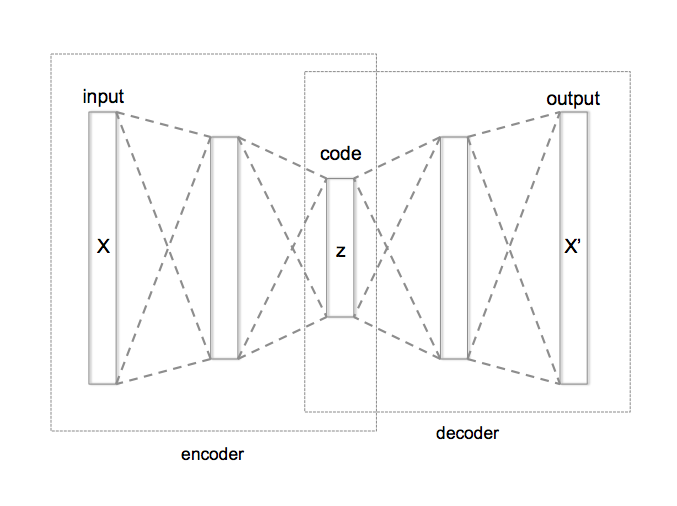
\includegraphics[width=0.6\textwidth]{images/figures/Autoencoder_structure.png}
    \caption{An undercomplete autoencoder has a latent code $z$ whose dimension is smaller than the 
    dimension of the input $x$.
    Image taken from \parencite{2015-Chervinskii-autoencoder}} \label{figure_undercomplete_ae}
\end{figure}

Undercomplete autoencoders can be used for pretraining by taking the trained encoder that has 
learned the most important features of the input and using it for the actual desired task like 
classification. Another obvious application would be dimensionality reduction.

\subsection{Kullback-Leibler Divergence} \label{KL-Divergence}

\subsubsection{Entropy}

A part of the loss function used in the variational autoencoder is based on Kullback-Leibler divergence.
To understand Kullback-Leibler divergence it seems necessary to explain entropy from
the field of information theory. In short, entropy is a measure for the minimum average size an
encoding for a piece of information can possibly have.

Suppose there is a system $S1$ that can have four different states $a, b, c, d$
and every one of those states is equally likely to occur, that means the probability $P(x)$
of each state $x$ is $1/4$. Now the goal is to losslessly transmit all information about that system
with the minimum average amount of bits. That can be done with only two bits for example like this

\begin{center}
    \begin{tabular} {c c c c}
        $a: 00$ & $b: 01$ & $c: 10$ & $d: 11$
    \end{tabular}
\end{center}

However, if $P(a)=1$ and $P(b)=P(c)=P(d)=0,$ zero bits will suffice to encode the information since
it is always certain that the system is in state a. So the entropy of the system clearly depends on
the probabilities of each state. To see in which way, one can consider the system $S2$ with 
$P(a)=1/2,\ P(b)=1/4,\ P(c)=1/8$ and $P(d)=1/8$. In that case it would be best to encode the state
with the highest probability with as few bits as possible since it has to be transmitted the most
often. That means $a$ is encoded with one bit as $0$. When decoding the information there must be
no ambiguities so while the encoding for $b$ has to start with a $1$ it cannot be $1$ since we need 
to encode two more states so $b: 10$. Additionally if $c: 11$ there would be no space left for $d$:
say $d: 111$ then if the transmitted information is $111111\dots$ it could either be decoded to
$ccc\dots$ or $dd\dots$. So $c$ should rather be encoded as $110$ which way $d: 111$ works. In the end a valid
encoding that can transmit all information with the minimum average amount of bits is

\begin{center}
    \begin{tabular} {c c c c}
        $a: 0$ & $b: 10$ & $c: 110$ & $d: 111$
    \end{tabular}
\end{center}

Here the states $c, d$ are encoded with three bits instead of the two bits in the first example.
But $c$ and $d$ are transmitted far less often than $a$ which now only needs one bit. To be more precise
half of all transmissions have one bit. Additionally a quarter of all transmissions have two bits. 
The sum of those probabilities multiplied with the respective amount of bits is the average amount of bits
needed to transfer the information in a given encoding. So in the example, with $f(x)$ as the number of
bits that encode a state $x$, that turns out to be $P(a)f(a)+P(b)f(b)+P(c)f(c)+P(d)f(d)=1.75$.
That means for $S2$ on average you only need $1.75$ bits to encode a state and since that is also the
minimum $1.75$ is the entropy of $S2$.

In general, when the encoding is optimal, $f(x)$ is the same as $\log_{2} \frac{1}{P(x)}$. For $S1$ $P(x)$ is $1/4$
so the number of bits for $x$ is $\log_{2} (4)=2$ which matches the two bits the first encoding uses 
for the states of $S1$.

The entropy $H$ of a system with a set of discrete events $X$ and the probability distribution $P(x)$
for each $x\in X$ is
\begin{equation}
    H(P)=\sum_{x\in X} P(x)\log_{2} \frac{1}{P(x)} = -\sum_{x\in X} P(x)\log_{2} P(x)
\end{equation}
This is often written as the expectation for a  given state $x$ under the distribution $P$.
\[ H(P)=E_{x\sim P}[-log_{2}P(x)]\]
Intuitively if a system has high entropy, the size of the encodings are high on average and many states
have small probabilities. This means it is hard to predict what state the system will be in at a given time
since there is no state that can be guessed with high confidence. If entropy is low, zero for example,
one can be confident that the system is in a certain state as in the previous example with $P(a)=1$.

%wie muss hier der fall P(x) = 0 abgesichert werden weil log(0) und 1/0 ?

\subsubsection{Cross Entropy}

If the real distribution $P$ of a system is unknown an estimate distribution $Q$ could be guessed
and encoding sizes $-log_{2}Q(x)$ can be produced which will not be optimal for the true distribution
$P$. Now with some data gathered and $P$ known the used encoding sizes can be cross-checked with the
expectation under the actual distribution resulting in the cross entropy $H(P,Q)$
\begin{equation}
    H(P,Q)=E_{x\sim P}[-log_{2}Q(x)]=-\sum_{x\in X} P(x)\log_{2} (Q(x))
\end{equation}
In machine learning tasks regarding classification this is often used as a loss function since the
label of a piece of data gives us a distribution $P$ with absolute certainty and $H(P)=0$. With the
inaccurate distribution $Q$ that the model estimates $H(P,Q)$ will be greater than zero unless
$P=Q$ where $H(P,Q)=H(P,P)=H(P)=0$. So the learning algorithm can try to minimize $H(P,Q)$.

\subsubsection{Kullback-Leibler Divergence}

Having computed the entropy $H(P)$ and cross-entropy $H(P,Q)$ of two distributions $P,\ Q$ it is 
possible to compare those distributions by comparing $H(P)$ and $H(P,Q)$ through subtraction
\begin{equation} \label{eq1}
    \begin{split}
        D_{KL}(P\parallel Q)    & = H(P,Q)-H(P) \\
                                & = E_{x\sim P}[-log_{2}Q(x)]-E_{x\sim P}[-log_{2}P(x)]\\
                                & = E_{x\sim P}[-log_{2}Q(x)+log_{2}P(x)]\\
                                & = E_{x\sim P}[log_{2}\frac{P(x)}{Q(x)}]\\
                                & = \sum_{x\in X} P(x)log_{2}\frac{P(x)}{Q(x)}
    \end{split}
\end{equation}
where $D_{KL}(P\parallel Q)$ is called the Kullback-Leibler divergence of $P$ and $Q$. This works
because $D_{KL}(P\parallel Q)$ is zero if $Q$ and $P$ are the same since that means $H(P,Q)=H(P)$.
On the opposite if $Q$ is different from $P$ then $H(P,Q)$ is greater than $H(P)$ and therefore 
the KL divergence is greater than zero proportional to how different $Q$ and $P$ are.
In summary Kullback-Leibler divergence is a measure of how different two probability distributions
are. The divergence is zero if the distributions are the same and greater than zero if not.

\subsection{Variational Autoencoders} \label{vae_background}

Standard autoencoders are fairly limited in their generative capabilities or in their capabilities
to interpolate in the latent space and the problem lies
in their latent code. For generation tasks a random latent code $z$ is sampled from the space of
possible latent codes. But with a standard autoencoder this space of possible latent codes is most
likely not continuous and chances are high that the sampled $z$ is intuitively speaking
from a gap in the latent space that the decoder has not been trained for. Therefore it will not
produce realistic outputs. This discontinuous latent space also means that interpolation in it
does not work well.

To solve this in a variational autoencoder the encoder does not produce discrete values but rather
probability distributions $p_{i}$ by generating two vectors of the same size as $z$ where one vector $\mu$
contains means and the other vector $\sigma$ contains standard deviations.
Then each $z_{i}$ is determined by sampling it from $p_{i}=N(\mu_{i},\sigma_{i})$.
As a result the decoder is forced to not 
only just learn how to decode single, discrete latent codes but also the possible variations
introduced by the random sampling. This leads to the desired continuous decodable latent space.
However, the encoder could still produce $\sigma$ sigma that are very small and $\mu$ that are far apart.
To prevent this the encoder is forced to produce distributions that are similar to a normal
distribution with standard deviation 1 and mean 0 by adding a second loss function next to the
loss $L(x,x')$ between the input and output.

As discussed in \ref{KL-Divergence} Kullback-Leibler divergence can be seen as a measure for the
difference of two probability distributions. This means that it can be used as the second loss
function for the variational autoencoder that should now also minimize the sum
of all the Kullback-Leibler divergences between the output distribution and $N(0,1)$.

To achieve the goal of generating new content that is similar to the input that the variational 
autoencoder was trained with, one can sample each component for a latent code from $N(0,1)$ and
use it as the input for the decoder.
Also smooth interpolation in the latent space is possible leading to possibilities for combining
content in interesting ways.

Further details about variational autoencoders can be found here \parencite{2016-doersch-tutorial}.

\subsection{t-Distributed Stochastic Neighbor Embedding} \label{t-sne}

The method t-distributed stochastic neighbor embedding (t-SNE) is a machine learning technique for reducing
dimensionality. It was first 
introduced by Laurens van der Maaten and Geoffrey Hinton \parencite{2008-vanDerMaaten-visualizing} who
claim that t-SNE would be especially well suited for creating single visualizations that reveal the 
structure of the high dimensional data. Their paper is also where most of the information for this 
subsection is drawn from.

The method generates an initial embedding in the low dimensional space by sampling from a normal distribution 
centered around the origin. The learning process improves this embedding by first calculating a 
representation of the similarities between all points in the high dimensional space. For the similarity of point
$x_{i}$ to $x_{j}$ this representation is a conditional probability $p_{ij}=\frac{r_{i|j} + r_{j|i}}{2N}$,
so the conditionals are symmetric, with 
$r_{i|j}$ given by the following.

\begin{equation} \label{pij}
    r_{i|j}=\frac{exp(-|x_{i}-x_{j}|^2/2\sigma_{i}^2)}{\sum_{k}\sum_{l\neq k} exp(-|x_{k}-x_{l}|^2/2\sigma_{i}^2)}
\end{equation}

For the similarity of points $y_{i}$ and $y_{j}$ from the low dimensional space the representation is a conditional
probability $q_{ij}$ given by the following.

\begin{equation} \label{qij}
    q_{ij}=\frac{(1 + -|x_{i}-x_{j}|^2)^{-1}}{\sum_{k}\sum_{l\neq k} (1 + -|x_{i}-x_{j}|^2)^{-1}}
\end{equation}

Then the mistake between the representation in high dimensional space and in low dimensional space is
given by the Kullback-Leibler divergence \ref{KL-Divergence} of high dimensional and low dimensional
conditionals which is $\sum_{i}\sum_{j\neq i}p_{ij}log \frac{p_{ij}}{q_{ij}}$.

The Kullback-Leibler divergence is then minimized with gradient descent, moving the points in the embedding to
a more optimal position.